\documentclass[a4paper, 12pt, notitlepage]{article}
\usepackage[margin=0.5in]{geometry}
\usepackage[utf8x]{inputenc}
\usepackage{fancyhdr}
\usepackage{amsmath}
\usepackage{amssymb}
\usepackage{gensymb}
\usepackage[makeroom]{cancel}
\usepackage{tikz}
\usepackage{float}
\usepackage{pdfpages}
\usepackage{graphicx}
\usepackage{tabularx}
\usepackage{hyperref}

\title{Computational Biology - 2$^\text{nd}$ Assignment}
\author{Nicolás Espinoza Muñoz}
\date{October 30, 2020}

\newcommand\numberthis{\addtocounter{equation}{1}\tag{\theequation}}
\pagenumbering{gobble}

\begin{document}
\maketitle
\subsubsection*{Introduction}
When calculating certain potential energy interactions, specifically in systems with many elements, one faces what is known as an N or Many-body problem, depending on the nature of said system. In our case we deal with a system made of many particles that interact in a classical fashion by way of electrostatics. When the particle ensembles become too large - that is, the system has too many components - calculating the interactions between all pairs directly becomes computationally demanding, or even outright impossible. Thus, many approximations have been developed, and in recent decades successfully applied, to accelerate the calculations of this kind while maintaining a good degree of precision. This text will focus on a specific method, or more accurately a pair off methods directly related: the Ewald Summation and the Particle-Mesh Ewald (PME) methods. First we will present the theory behind the Ewald Summation and PME, and afterwards we will compare the calculation times and precision of said methods with a direct calculation, and prove that the theoretical foundation holds true for the power of the acceleration algorithms.
\section*{Electrostatic theoretical outline}
The electrostatic interactions between particles are calculated for all particles in a system. Since a single reference particle is affected by all other components of the system, and one has to cycle through all of said components as reference to obtain the electrostatic potential of the ensemble, this calculation is of order $\mathcal{O}(N^2)$. However, there are acceleration methods that help achieve the results needed much faster, but at the expense of a bit of precision. For starters we will present the basic electrostatic potential formula, which is the basic way of calculating interactions, and the one that grows as $\mathcal{O}(N^2)$. In the same section, the Ewald Summation and PME methods will be introduced. Finally, a comparison between methods will be shown so as to appreciate the differences between them, and the benefits of acceleration algorithms.
\section{Direct Calculation}\label{sec:DC}
For a system like the one shown in Figure \ref{fig:fig_omega}, interactions are calculated in pairs, then summed over all possible pairs for a specific $i$ particle interacting with all $j$, and summed again for all $i$ particles in the ensemble.
\begin{equation}
E = \frac{1}{2}\sum_{i = 1}^{N}\sum_{\substack{j=1\\j\neq i}}^{N}\frac{1}{4\pi\varepsilon}\frac{q_i\cdot q_j}{|\mathbf{r}_i - \mathbf{r}_j|}\quad \implies \quad E = \frac{1}{2}\sum_{i=1}^{N}q_i\cdot\phi(\mathbf{r}_i)\label{eq:eq1}
\end{equation}
For a continuous charge distribution one has to integrate over the volume of interest and afterwards proceed with the double summations, but the procedure stays the same.
\begin{figure}
	\centering
	\vspace{100pt}
	\input{./Figures/scheme.eps_tex}
	\caption{Sketch of a system of interacting particles.}\label{fig:fig_omega}
\end{figure}
It will become useful to introduce the Poisson equation of electrostatics, after which one can calculate the potential in terms of the charge density
\begin{equation}
	-\nabla^2\phi = \frac{\rho}{\varepsilon}\label{eq:eq2}
\end{equation}
There's not much more to elaborate on this, except for the fact that it is easy to see how the computation time escalates with the square of the number of particles $N$. With periodic boundary conditions this is obviously impossible to calculate, because it would mean an infinite double summation. So instead we proceed with the Ewald Summation method.
\section{Ewald Summation}\label{sec:ES}
The Ewald Summation takes a slowly converging potential, and splits it into two parts: a short range one and a long range one. For this, one starts by actually splitting the charge density $\rho$, and adding a zero via a Gaussian distribution
\begin{equation}
\rho_i = \rho_i^S + \rho_i^L = q_i\delta(\mathbf{r} - \mathbf{r}_i) - q_i G_\sigma(\mathbf{r} - \mathbf{r}_i) + q_i G_\sigma(\mathbf{r} - \mathbf{r}_i)\label{eq:eq3}
\end{equation}
where
\begin{align*}
&\rho_i^S = q_i\delta(\mathbf{r} - \mathbf{r}_i) - q_i G_\sigma (\mathbf{r} - \mathbf{r}_i)\\
&\rho_i^L = q_i G_\sigma (\mathbf{r} - \mathbf{r}_i)
\end{align*}
So using Equation (\ref{eq:eq3}) into Equation (\ref{eq:eq2}) to obtain a split potential ($\phi^S$ and $\phi^L$), we get
\begin{gather*}
	\phi_i^S = \sum_{\substack{j=1\\j\neq i}}^{N}\frac{q_j}{4\pi\varepsilon}\int\frac{\delta(\mathbf{r}_i - \mathbf{r}') - G_\sigma (\mathbf{r}_i - \mathbf{r}')}{|\mathbf{r}_i - \mathbf{r}'|}\, dV'\\
	\phi_i^L = \sum_{\substack{j = 1\\j\neq i}}^{N}\frac{q_j}{4\pi\varepsilon} \int \frac{G_\sigma(\mathbf{r}_i - \mathbf{r}')}{|\mathbf{r}_i - \mathbf{r}'|}\, d V' \numberthis \label{eq:eq4}
\end{gather*}
The first integral of Equation (\ref{eq:eq4}) corresponds to the $erfc(x) = 1 - erf(x)$, the error function complement, and the second integral is the error function itself. The logic behind this procedure is that the short range potential is singular, but converges quickly. The long range potential on the other hand is not singular, and accounts for the slowly converging nature of the actual physical potential, and the sum of both returns the original $\phi$.\\\\
So since the short range potential converges quickly, we can calculate it directly, which leaves the long range potential as the only actual dilemma. For this, one can apply a Fourier Transform to obtain the potential in reciprocal space - that is, in terms of frequencies. By transforming the charge density to Fourier Space, we can easily calculate the long range potential
\begin{gather*}
	\mathcal{F} (\rho) = \hat{\rho} = \int\rho^L\, e^{-i\mathbf{k}\cdot\mathbf{r}}\, dV\\
	\mathcal{F} (\phi) = \hat{\phi} = \int\phi^L \, e^{-i\mathbf{k}\cdot\mathbf{r}}\, dV
\end{gather*}
So to calculate the long range potential in real space, one calculates it in reciprocal space first by applying the equivalent form of Equation (\ref{eq:eq2})
\begin{equation}
	\hat{\phi}^L = \frac{\hat{\rho}^L}{\varepsilon |\mathbf{k}|^2}\label{eq:eq5}
\end{equation}
And then use the inverse Fourier Transform to recover the real space version of the result. The factor $1/|\mathbf{k}|^2$ in Equation (\ref{eq:eq5}) comes from the Laplace operator applied to the potential, and $\mathbf{k}$ is  the reciprocal vector. The idea behind working in Fourier Space is that the summation for $\phi^L$ is actually short range in reciprocal space, so one can calculate it with few terms in the summation to a decent precision. The resulting expression for the real form of the long range potential is
\begin{equation}
	\phi^L = \frac{1}{V}\sum_{k=1}\hat{\phi}^L e^{i\mathbf{k}\cdot\mathbf{r}}= \frac{1}{V\varepsilon}\sum_{k = 1}\sum_{j = 1}^N \frac{q_j}{|\mathbf{k}|^2}e^{i\mathbf{k}\cdot(\mathbf{r} - \mathbf{r}_j)}e^{\beta}\label{eq:eq6}
\end{equation}
Where $\beta = -\sigma^2|\mathbf{k}|^2/2$, and $\sigma$ is the standard deviation of the error function.
Finally, we sum both long and short range potentials to recover the original, physical potential. This method, as is, converges with $\mathcal{O}(N^{3/2})$, but it can be accelerated by means of the Fast Fourier Transform instead of a regular one for calculating the potential in reciprocal space. This makes the method a lot faster for big $N$, and the calculation time escalates with order $\mathcal{O}(N\log N)$; for this we have to explain the PME method, which makes use of the FFT acceleration algorithm.
\section{Particle-Mesh Ewald}\label{sec:PME}
The PME method bases its application in the fact that, usually, one works with regular meshes rather than the specific particles, and for Periodic Boundary Conditions, the number of mesh elements will more likely than not be smaller than the number of particles interacting. The method consists of distributing the charge of a particle onto the mesh. The potential is then calculated in Fourier Space on the mesh points by applying the FFT\footnote{A regular grid is a requirement for the common FFT to work. Other methods that work on triangular meshes are being developed, but we will stick to the typical situation here.}, and brought back to real space by means of the inverse Fast Fourier Transform. Figure \ref{fig:fig1} shows the idea in a 1-D setting, using a Gaussian distribution of the charge, but the distribution itself may vary. As stated in the previous section, PME is of order $\mathcal{O}(N\log N)$.
\begin{figure}[h]
	\centering
	\input{./Figures/PME.eps_tex}
	\vspace{2.5pt}
	\caption{Distribution example for a one-dimensional test charge.}\label{fig:fig1}
\end{figure}

\section*{Comparison between calculation methods}
We shall proceed with a comparison between the methods presented in sections \ref{sec:DC}, \ref{sec:ES} and \ref{sec:PME}. For this, we used three ``boxes" with regular sides: $3.0\text{, }4.0\text{, }6.0$ [nm]. The cutoff length used is $2.0$ [nm], the error tolerance\footnote{According to documentation: \textit{The error tolerance is roughly equal to the fractional error in the forces due to truncating the Ewald summation.}} for the force calculation is set to $10^{-3}$ and the number of steps in the simulation was 200.
\begin{figure}[H]
	\centering
	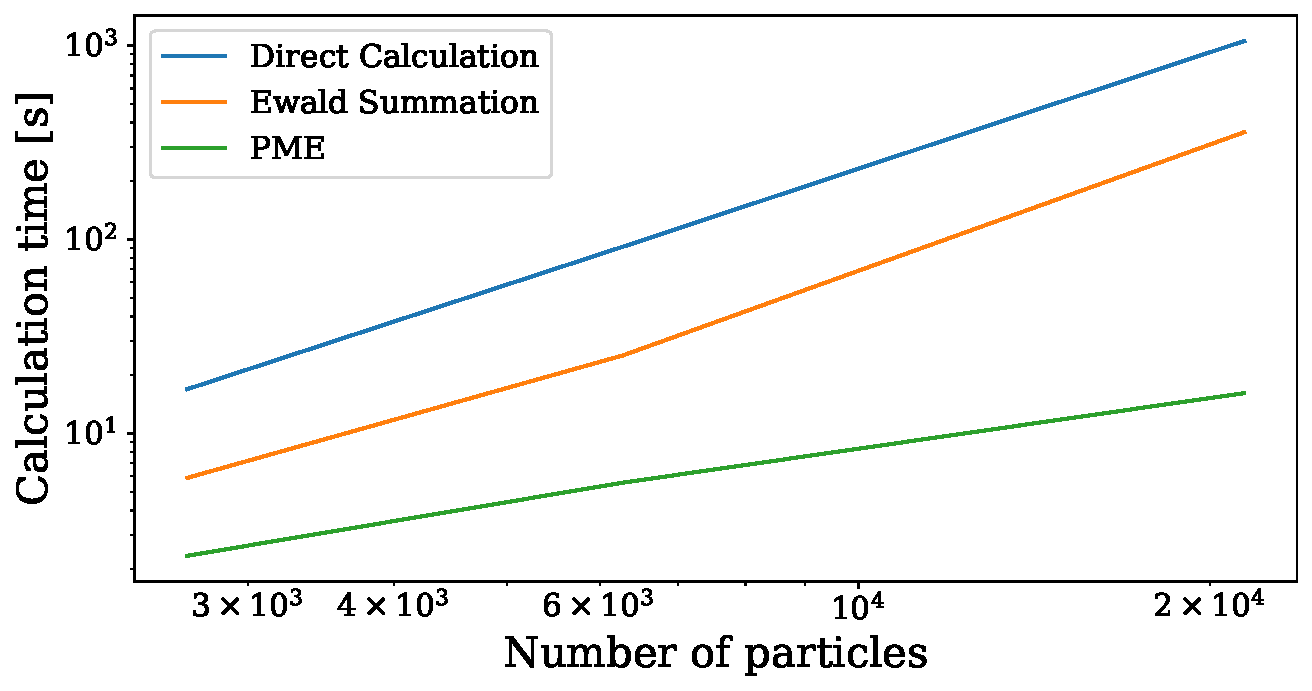
\includegraphics[scale=0.5]{./Figures/plot1.pdf}
	\caption{Comparison in the convergence time of the three tested methods.}\label{fig:fig2}
\end{figure}
\noindent
We worked with three points due to the limitations of computing on a notebook, as times would really escalate too much. In Figure \ref{fig:fig2} we show a plot of calculation times as a function of the size of the system. Since the program fits as many molecules as it can in a box, the bigger the box, the more particles in the system. We appreciate a similarity between the direct calculation and Ewald Summation methods, which is correct according to theory, since a logarithmic scale plot can't really represent well enough the difference between $\mathcal{O}(N^2)$ and $\mathcal{O}(N^{3/2})$. When we look at the PME however, we can see that it clearly deviates from a strictly exponential behavior. This also makes sense and is in good agreement with theory, as PME calculation times are of order $\mathcal{O}(N\log N)$.\\\\
We have already shown the calculation times, but to us it seems correct to actually compare the numerical results of the potential energy calculation as well. That is shown in the next plot (Figure \ref{fig:fig3}), where it can be seen that both acceleration methods actually suffer quite a lot in contrast with the direct calculation, since this is the analytical form of calculating the potential.
\begin{figure}
	\centering
	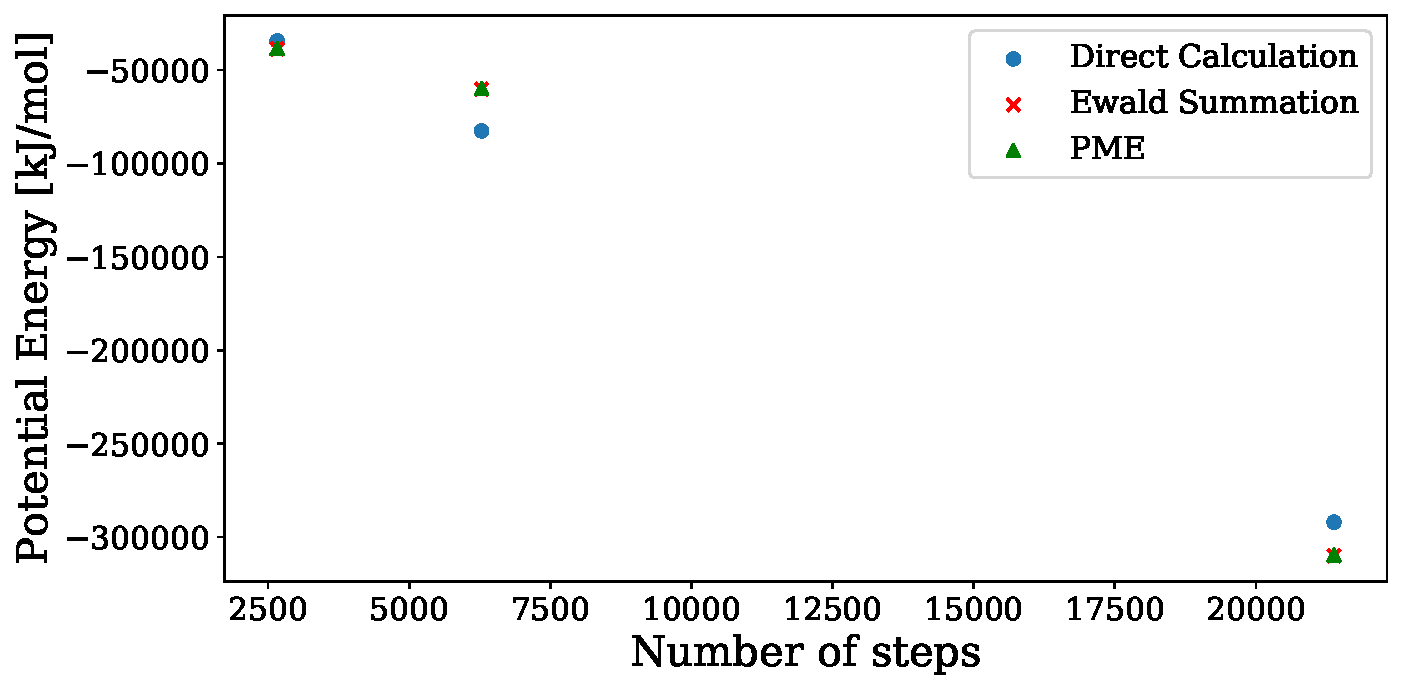
\includegraphics[scale=0.5]{./Figures/plot2.pdf}
	\caption{Comparison of the energy calculation result of the three tested methods.}\label{fig:fig3}
\end{figure}
This is attributed to the error tolerance established for the calculations, as well as to the cutoff parameter. Nevertheless, one is not supposed to apply the acceleration methods on small problems, and therefore we present the relative error for the biggest system simulated; the value for $N = 21384$ particles is $err = 6.2$\%, and it decreases as the size of the ensemble of particles gets bigger. We also tried adjusting the \textit{error tolerance} parameter, and set it to $5\times 10^{-4}$. In Figure \ref{fig:fig4} the corresponding results are presented.
\begin{figure}
	\centering
	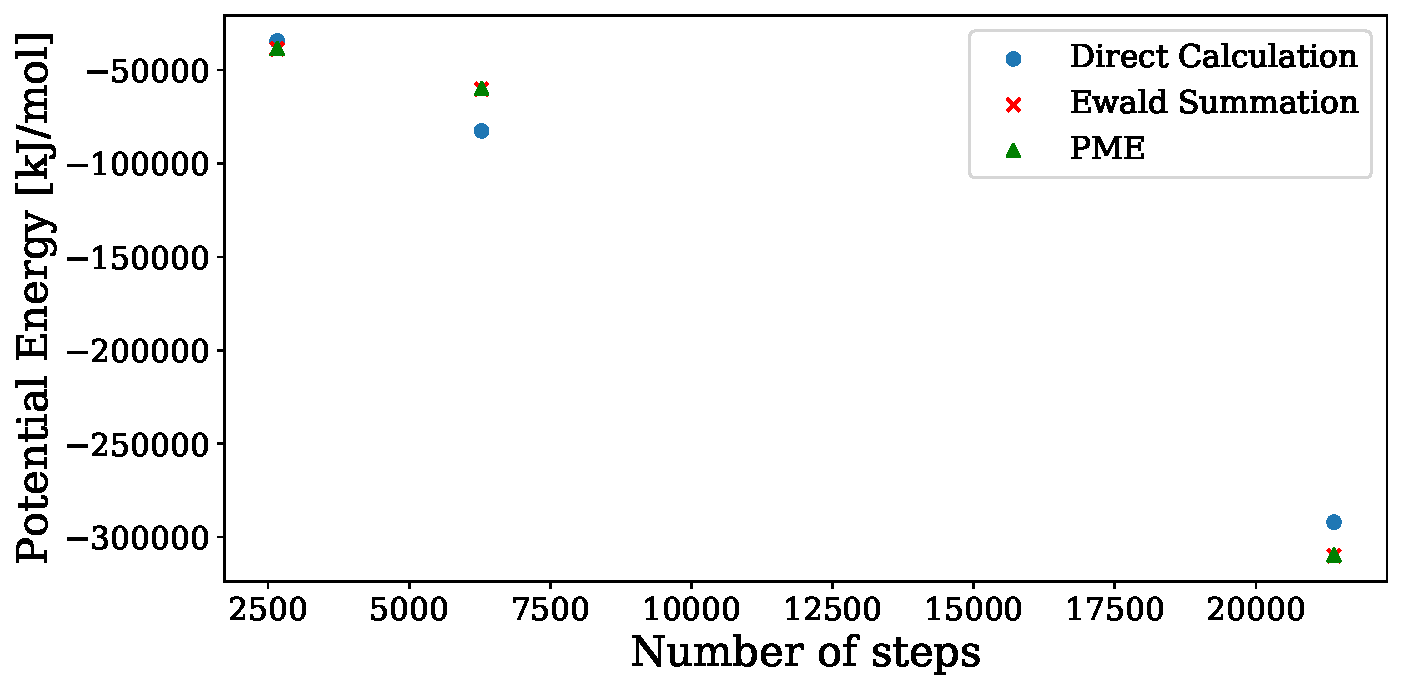
\includegraphics[scale=0.35]{./Figures/plot3.pdf}\hspace{15pt}
	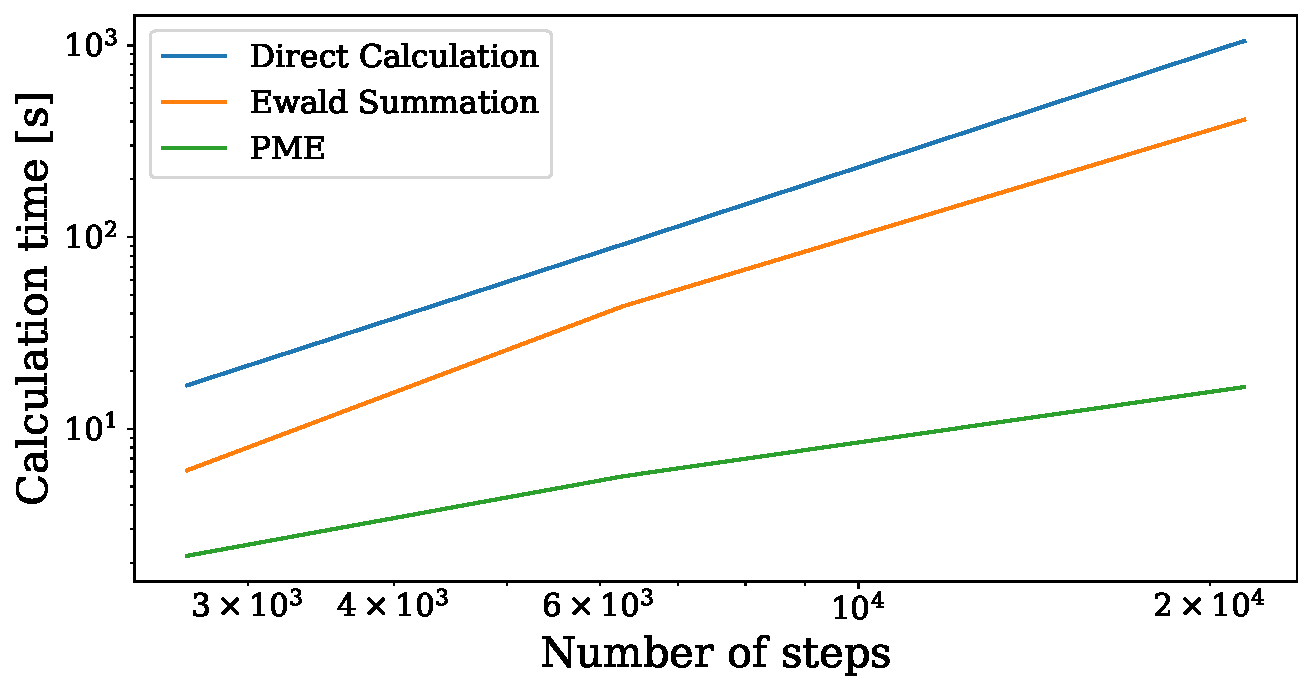
\includegraphics[scale=0.35]{./Figures/plot4.pdf}
	\caption{Effect of the error tolerance variable in the performance of the Ewald Summation and PME method}\label{fig:fig4}
\end{figure}
The behavior is the same, so the effect of the error tolerance is small and can be discarded as a major factor in the calculation precision, but not so in the calculation times of the Ewald Summation method. For the biggest system simulated, said method had an increase in calculation time of $14$\%, and the potential energy varied in only $0.2$\%, when changing the tolerance from $10^{-3}$ to $5\times 10^{-4}$.
\subsection*{Conclusions}
As it stands, we have simulated three sets of systems with three different calculation methods. After experimenting with the simulation setting given, there is hardly a more important conclusion than the advantage that represents the PME method. After many tests, most of which are not shown here, we have witnessed how the accelerated methods for non-bonded interactions help decrease the calculation times greatly, especially as the size of the ensemble gets bigger and therefore the amount of interactions increases. The trade-off is in terms of precision, but this difference in comparison with a direct calculation rapidly vanishes, especially if weighed against the gain in calculation time when simulating huge systems.\\\\
As a final remark, the analysis of the cutoff parameter was left out of this text, because we saw that, even though the actual values were clearly not equal, the tendency was pretty much the same for the tested values of $2.5$ [nm] and $1.5$ [nm]; this happened for both the potential energy - which changed in $<1\%$ - and the calculation time.

\begin{thebibliography}{5}
	\bibitem{Jackson}
	Jackson, J. D. \textit{Classical Electrodynamics}, Third Edition; Wiley, 1998
	\bibitem{Cai}
	Lee, H.; Cai, W. \textit{Ewald Summation for Coulomb Interactions in a Periodic Supercell}, 2009
	\bibitem{openmm}
	\href{http://docs.openmm.org/latest/userguide/application.html}{http://docs.openmm.org/latest/userguide/application.html}
\end{thebibliography}
\end{document}